\documentclass[Main.tex]{subfiles}

\begin{document}
	%-=-=-=-=-=-=-=-=-=-=-=-=-=-=-=-=-=-=-=-=-=-=-=-=
	%
	%	CHAPTER
	%
	%-=-=-=-=-=-=-=-=-=-=-=-=-=-=-=-=-=-=-=-=-=-=-=-=
	
	\chapter{Describing Relationships}
	
	%-=-=-=-=-=-=-=-=-=-=-=-=-=-=-=-=-=-=-=-=-=-=-=-=
	%	SECTION:
	%-=-=-=-=-=-=-=-=-=-=-=-=-=-=-=-=-=-=-=-=-=-=-=-=
	
	\section{Scatterplots and Correlation}\index{Scatterplots and Correlation}

	\begin{example}[Scatterplots]\index{Scatterplots} \hfill \\
		\begin{itemize}
			\item A \textbf{scatterplot} displays the relationship between two quantitative variables measured on the same individuals.\\
			\item Explanatory and response variable:
				 \begin{subequations}
				 	\begin{align}
				 	\begin{cases}
				 	\text{$x$$\Longrightarrow$ \textbf{Explanatory variable}}\\
				 	\text{$y$$\Longrightarrow$ \textbf{Response variable}}
				 	\end{cases}
				 	\end{align}
				 \end{subequations}			
		\end{itemize}
	\end{example}
	
	\begin{example}[Describing Scatterplots]\index{Describing Scatterplots} \hfill \\
		\begin{itemize}	
			\item \textbf{Describing Scatterplots}
		\end{itemize}		
				 \begin{subequations}
				 	\begin{align}
				 	\text{Scatterplots}				 	
				 	\begin{cases}
				 	\text{\textbf{Direction} (gengeral point trend)}
					 	\begin{cases}
					 	\text{up to right: positive association}\\
					 	\text{down: negative association}
					 	\end{cases}	\hfill \\ \\				 	
				 	\text{\textbf{Form} (shape of direction)}				 	
					 	\begin{cases}
					 	\text{Linear}\\
					 	\text{Curved}
					 	\end{cases}	\hfill \\ \\						 		
				 	\text{\textbf{Strength} (how closely graph fits form)}				 	
					 	\begin{cases}
					 	\text{Strong}\\
					 	\text{Weak}\\
					 	\end{cases}\hfill \\ \\					
					\text{\textbf{Outlier} (a departure falls outside the overall relationship)}						 					 			 	
				 	\end{cases}
				 	\end{align}
				 \end{subequations}					
	\end{example} \hfill \newpage
	
	\begin{example}[Measuring Linear Association]\index{Measuring Linear Association} \hfill \\
		\begin{itemize}	
			\item The \textbf{correlation $r$} measures the direction and strength of the linear relationship between two quantitative variables.
			
			\begin{figure}[H]
				\centering
				\includegraphics[height=8.5cm,width=13cm]{correlation}
				\caption{Plots with different correlations}
				\label{correlation}
			\end{figure}
					
			\begin{definition}[Correlation]\index{Correlation}
			 	\begin{subequations}
			 		\begin{align}
			 		r&=\frac{Z_{x_{1}}Z_{y_{1}}+Z_{x_{2}}Z_{y_{2}}+\cdots+Z_{x_{n}}Z_{y_{n}}}{n-1}\\
			 		&=\frac{1}{n-1}\sum^{n}_{i=1}(\frac{x_{i}-\bar{x}}{S_{x}})(\frac{y_{i}-\bar{y}}{S_{y}})\\
			 		&=\frac{1}{n-1}\sum Z_{x}Z_{y} \qquad (Z=\frac{x_{i}-\bar{x}}{S_{x}})	\hfill	
				 	\end{align}
			 	\end{subequations}				
			\end{definition}\hfill %\\			

			\item \textbf{Features of Correlation:}\\
				\begin{itemize}									 	
					\item $r=1\Longrightarrow$ \textbf{linear}, perfect positive correlation.\\
					\item $r>0\Longrightarrow$ \textbf{positive} association.\\
					\item $r<0\Longrightarrow$ \textbf{negative} association.\\
					\item $r=-1\Longrightarrow$ \textbf{linear}, perfect negative correlation.\\
					\item $r=0\Longrightarrow$ \textbf{doesn't} guarantee there's \textbf{no} relationships between two variables, just \textbf{No} linear relationship.\\
					\item \textbf{only} measures the strength of a \textbf{linear relationship}.\\
					\item can \textbf{Not} conclude that change in one variable cause in the other.\\
					\item is the \textbf{same} when you \textbf{inverse} $x$ and $y$.\\
					\item is the \textbf{same} when you change the unit.\\ \emph{e.g}: height in inches or meters, weight in pounds or kilograms.\\
					\item is \textbf{Not} resistant to outliers.\\
					\item is \textbf{Not} a complete summary of two-variable data.\\
					\item both variables must be \textbf{quantitative}.						 	
				\end{itemize}				
		\end{itemize}	
	\end{example} \hfill
						
	%-=-=-=-=-=-=-=-=-=-=-=-=-=-=-=-=-=-=-=-=-=-=-=-=
	%	SECTION:
	%-=-=-=-=-=-=-=-=-=-=-=-=-=-=-=-=-=-=-=-=-=-=-=-=
	
	\section{Least-Squares Regression}\index{Least-Squares Regression}
	
	\begin{exercise}[Regressions]\index{Regressions} \hfill \\
			\begin{itemize}
				\item A \textbf{Regression line} is a line that describes how a response variable $y$ changes as an explanatory variable $x$ changes.
				
					\begin{definition}[Regression line, predicted value, slope, $y$ intercept]\index{Regression line, predicted value, slope, $y$ intercept}\hfill \\						
						A \textbf{regression line} relating $y$ to $x$ has an equation of the form:
							\begin{subequations}
								\begin{align}
								\hat{y}=a+bx
								\end{align}
							\end{subequations}
						\begin{itemize}
							\item $\hat{y}$ is the \textbf{predicted value}.
							\item $b$ is the \textbf{slop}.
							\item $a$ is the \textbf{$y$ intercept} ($y$ value when $x=0$).\hfill
						\end{itemize}
					\end{definition}\hfill %\\					
				\item \textbf{Extrapolation} is the use of regression line for prediction far outside the interval of values of the explanatory variable $x$ used to obtain the line.
			\end{itemize}		
	\end{exercise}
	
	\begin{exercise}[Residuals and the Least-Squares Regression Line]\index{Residuals and the Least-Squares Regression Line} \hfill \\
		\begin{itemize}	
			\item A \textbf{residual} is the difference between an observed value of the response variable and the value predicted by the regression line.
				
				\begin{definition}[Residual]\index{Residual}
					\begin{subequations}
						\begin{align}
						\text{residual}&=\text{observed $y$}-\text{predicted $y$}\\ \notag
						&=y-\hat{y}
						\end{align}
					\end{subequations}
				\end{definition}\hfill \\

			\item The \textbf{least-squares regression line} of $y$ on $x$ is the line that makes the sum of the squared residuals as small as possible.
			
				\begin{definition}[Least-squares regression line]\index{Least-squares regression line}\hfill \\ \hfill 
					\begin{subequations}
					\text{The least-squares regression line is the line $\hat{y}=a+bx$ with \textbf{slope}}
						\begin{align}
						b=r\frac{s_{y}}{s_{x}}
						\end{align}
					\text{and \textbf{$y$ intercept}}
						\begin{align}
						a=\bar{y}-b\bar{x}
						\end{align}
					\text{The least-squares regression line always passes through the point ($\bar{x},\bar{y}$)}
					\end{subequations}
				\end{definition}
									
			\begin{figure}[H]
				\centering
				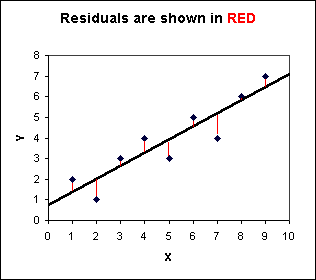
\includegraphics[height=4.7cm,width=7cm]{LSRegression}
				\caption{A Least-squares regression line}
				\label{Least-squares regression line}
			\end{figure}
			
			\item A \textbf{residual plot} is a scatterplot of the residuals against the explanatory variable, helping us access whether a linear model is appropriate.	
			
			\begin{figure}[H]
				\centering
				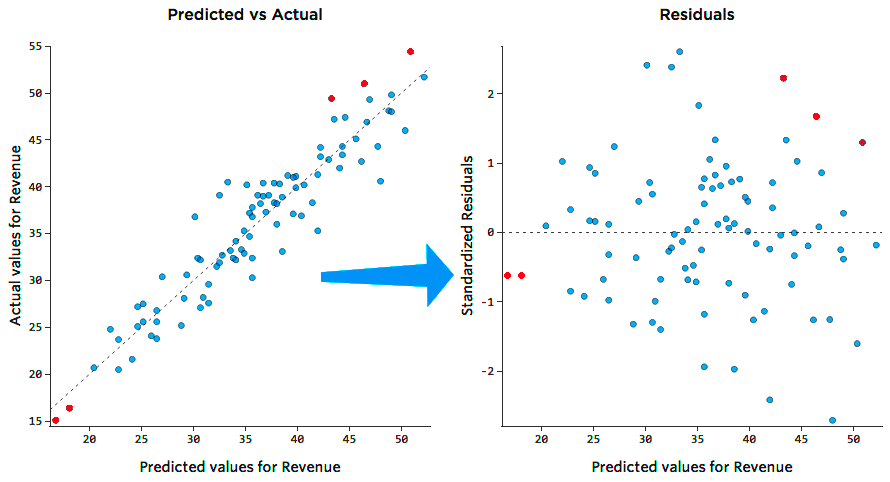
\includegraphics[height=7cm,width=14cm]{residualplot}
				\caption{A residual plot}
				\label{residual plot}
			\end{figure}			
		\end{itemize}
	\end{exercise} \hfill
	
	\begin{exercise}[The Role of $s$ and $r^{2}$ in Regression]\index{The Role of $s$ and $r^{2}$ in Regression} \hfill \\
		\begin{itemize}	
			\item If we use a least-squares line to predict the values of a response variable $y$ from an explanatory variable $x$, the \textbf{standard deviation of the residuals} $s$ is
			
				\begin{definition}[Standard deviation of the residuals $s$]\index{Standard deviation of the residuals $s$}
					\begin{subequations}
						\begin{align}
						s=\sqrt{\frac{\sum\text{residuals}^{2}}{n-2}}=\sqrt{\frac{\sum(y_{i}-\hat{y})^{2}}{n-2}}
						\end{align}
					\end{subequations}
				\end{definition} \hfill
				
			This value gives the approximate size of a typical \textbf{prediction error} (residual)\\
			
			\item The \textbf{coefficient of determination} $r^{2}$ is the fraction of the variation in the values of $y$ that is accounted for by the least-squares regression line of $y$ on $x$.\hfill \\
			(The \textbf{percentage} of how well the line fits those data)
			
				\begin{definition}[Coefficient of determination  $r^{2}$]\index{Coefficient of determination $r^{2}$}
					\begin{subequations}
						\begin{align}
						r^{2}=1-\frac{\sum\text{residuals}^{2}}{\sum(y_{i}-\bar{y})}=1-\frac{\sum(\text{Obs$-$prediction})^{2}}{\sum(\text{Obs$-$mean Obs})^{2}}
						\end{align}
					\end{subequations}
				\end{definition} \hfill						
		\end{itemize}
	\end{exercise}
	
	\begin{exercise}[Outliers and influential observations in regression]\index{Outliers and influential observations in regression} \hfill \\
		\begin{itemize}
			\item An \textbf{outlier} is an observation that lies outside the overall pattern of the other observation. Points that are outliers \underline{in the $y$ direction} but not the $x$ direction of a scatterplot have \underline{large residuals}. Other outliers may not have large residuals.\\
			\item An observation is \textbf{influential} for a statistical calculation if removing it would markedly change the result of the calculation. \underline{Outliers in $x$} are often influential for the regression line.
		\end{itemize}
	\end{exercise}		
\end{document}